\documentclass[draft,linenumbers]{agujournal2018}
\usepackage{apacite}
\usepackage{url} % should fix any errors with URLs in refs.
\usepackage{amsmath}
\usepackage{url}
%\usepackage{xcolor}
%\usepackage[colorlinks]{hyperref}
\usepackage[colorinlistoftodos]{todonotes}
\draftfalse

%\journalname{Space Weather}

% Journal options
% https://docs.google.com/document/d/1hGGISS5dM__oSUb8JVXcjPFPBdVrGD_LNnkflubR6xw/edit

\newcommand{\citeay}[1]{%
\citeauthor{#1}, \citeyear{#1}%
}

\begin{document}

\title{The Magnetotelluric Impedance at Middelpos, South Africa}

\authors{R.S. Weigel\affil{1} and P.J. Cilliers\affil{2}}

\affiliation{1}{Space Weather Lab, George Mason University}
\affiliation{2}{South African National Space Agency}

\affiliation{1}{4400 University Drive, Fairfax VA 22030}
\affiliation{2}{Hospital Street, Hermanus 7200}

\correspondingauthor{R.S. Weigel}{rweigel@gmu.edu}

\begin{keypoints}
\item 
\item 
\item 
\end{keypoints}

\begin{abstract}
From 2012-07-12 through 2012-11-07 (119 days), a magnetotelluric (MT) instrument made continuous 1-second recordings at a Middelpos, South Africa site.
\end{abstract}

\section{Introduction}

\section{Data}
\label{section:Data}

Data were obtained from the LEMI-417\todo{ref} instrument, which is designed for long--term recording of MT data; it is comprised of a 3--axis fluxgate magnetometer and a 2--axis electric field antenna. The instrument was installed in an empty field near the small town (population $\sim$300) Middelpos, South Africa, located at geographic latitude -31.90605713$^\circ$ and longitude $20.23408023^\circ$ at an altitude of 1165~m. The instrument is powered by batteries that are charged from a solar panel. The instrument at Middelpos is one of eight such MT instruments in Southern Africa.

The $+x$-axes of both the magnetometer and electric field probe are aligned with geomagnetic North; the magnetic declination at Middelpos on 2012-07-12 was $-23.2541323^\circ$ (computed using the IGRF model [\cite{igrf}]). Figure~\ref{fig:site} shows an annotated Google Earth image of the instrument location and the electric field probes. The timestamp of the data is derived from a GPS chip that is part of the LEMI-417 instrument. Data were retrieved manually by a site visit by South African Space Agency (SANSA) technicians. 

\begin{figure}[h]
  \centering
  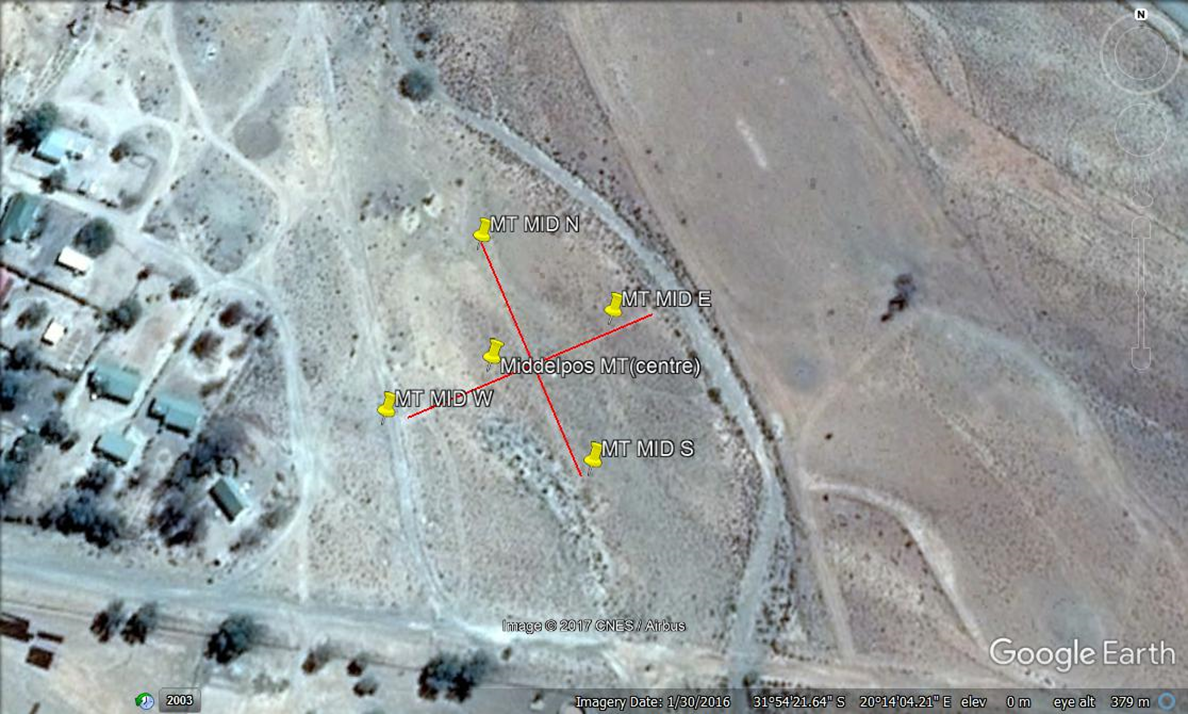
\includegraphics[width=\textwidth]{figures/site.png}
  \caption{Layout of the electric field sensors for the Middelpos MT Station. MID N, MID S, MID E, and MID W indicate the locations of the electric field electrodes. The distance between each pair of electrodes is $100$~m. The LEMI-417 unit is located at the crossing of the two electric field legs. The magnetometer was positioned $5$~m from the electronics to reduce the impact of the currents in the LEMI-417 instrument on the magnetometer measurements. 
}
 \label{fig:site}
\end{figure}

The time series of 1--second--cadence electric, $\mathbf{E}(t)$, and magnetic $\mathbf{B}(t)$, field measurements is shown in Figure~\ref{fig:timeseries}. Each component $k=x, y$ of the $\mathbf{E}(t)$ measurements was despiked by finding times when $E_k(t+1)-E_k(t)\ge 0.1$~mV/km and replacing values in the time range $[t-1, t+5]$ with linearly interpolated values based on $E_k(t-2)$ and $E_k(t+6)$. The number of spikes in $E_x$ was $X$\todo{insert value} ($X$\%)\todo{insert value}; for $E_y$, the number was $X$ ($X$\%).

The amplitudes of the Fourier coefficients for each vector component of the time series shown in Figure~\ref{fig:timeseries} are shown in Figure~\ref{fig:dft}. The amplitudes shown are frequency--domain band averages of the discrete Fourier transform amplitudes. The values of the band centers, marked with filled circles, the number of values in each band, and the band boundaries are given in Table~\ref{table:evaluationperiods} of the Appendix. The vertical bars correspond to 95\% confidence intervals; the length of the confidence interval for the magnitude of a Fourier coefficient, $\Delta|\widetilde{A}|$ was computed using $(1/|\widetilde{A}|)\sqrt{[A_r\Delta A_r]^2 + [A_i\Delta A_i]^2}$, where $\Delta A_r$ and $\Delta A_i$ are the 95\% confidence interval lengths for the real ($A_r$) and imaginary ($A_i$) parts of $\widetilde{A}$, respectively; $\widetilde{A}$ is one of $\widetilde{B}_x$, $\widetilde{B}_y$, $\widetilde{E}_x$, and $\widetilde{E}_y$, which are frequency-- domain averages shown in Figure~\ref{fig:dft}.

\clearpage

\begin{figure}[h!]
  \centering
  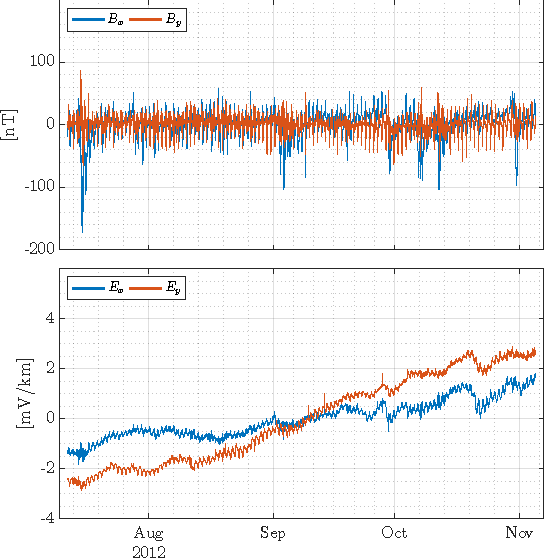
\includegraphics[width=0.65\textwidth]{figures/tsplot-original-Middelpos-tf1.pdf}
  \caption{Measurements used for analysis after mean subtraction and despiking.}
  \label{fig:timeseries}
\end{figure}

\begin{figure}[h!]
  \centering
  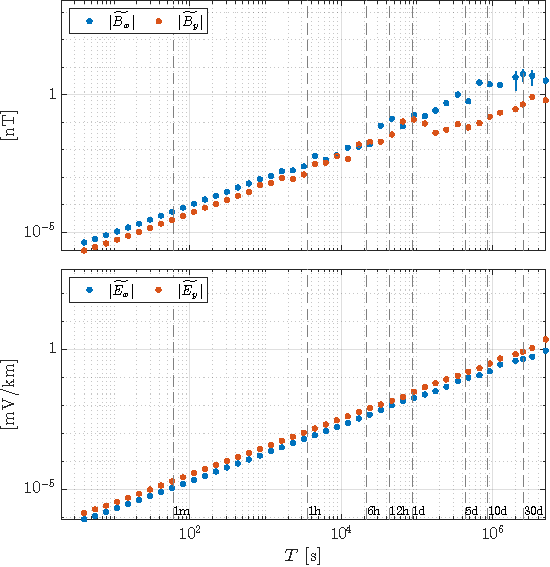
\includegraphics[width=0.65\textwidth]{figures/dftplot-original-averaged-magnitudes-Middelpos-tf1.pdf}
  \caption{Magnitudes of discrete Fourier transform coefficients for measurements in Figure~\ref{fig:timeseries}.}
  \label{fig:dft}
\end{figure}

\clearpage

\section{Models and Methods}
\label{section:Models_and_Methods}

$\mathbf{E}(t)$ and $\mathbf{B}(t)$ measurements are used to solve for the transfer function $\boldsymbol{\mathcal{Z}}$ in

\begin{linenomath*}
    \begin{equation}
        \mathbf{E}(f_e) = \boldsymbol{\mathcal{
    Z}}(f_e)\mathbf{B}(f_e)\text{ ,}
    \end{equation}
\end{linenomath*}

\noindent where $f_e$ is an ``evaluation frequency" and
    
\begin{linenomath*}
    \begin{equation}
        \boldsymbol{\mathcal{Z}}(f_e) = 
            \begin{bmatrix}
                Z_{xx}(f_e) & Z_{xy}(f_e)\\
                Z_{yx}(f_e) & Z_{yy}(f_e)
            \end{bmatrix}
    \end{equation}
\end{linenomath*}

\noindent using a method described by \citeay{Sims1971}: for each component $k=x,y$, a four parameter over--determined linear regression is performed using

\begin{equation}
E_k(f) = Z_{kx}(f)B_x(f) + Z_{ky}(f)B_y(f)
\end{equation}

\noindent with values of $f$ in a band around $f_e$. (The number of parameters is four because each component of $\boldsymbol{\mathcal{Z}}$ is complex \citep{Egbert1986}).

There are two general methods for computing estimates of $Z_{kx}$ and $Z_{ky}$ for each evaluation frequency: (1) compute the Fourier coefficients using the full time series and then perform a regression using Fourier coefficients in a band centered on the evaluation frequency and (2) split the full time series into (possibly overlapping) segments, perform a regression in a band centered on the evaluation frequency, and then average the segment estimates of $Z_{kx}$ and $Z_{ky}$. In this paper, we present results from both methods; for the second method, non--overlapping time series segments were used, and the estimates of $Z_{kx}$ and $Z_{ky}$ are unweighted averages. 

For the components of $\boldsymbol{\mathcal{Z}}$ computed using one $116$--day segment, the standard error was computed using\todo{}. For the magnitudes computed using $116$ $1$--day segments, the standard error was computed using the formula given in Section~\ref{section:Data} for the magnitudes of the DFT amplitudes. The error bars for the phases were computed using\todo{}.

(In addition, two methods have been used for computing the Fourier coefficients -- one uses the standard DFT formula, typically implemented using the FFT algorithm, and the other uses ``Cascade Decimation" \citep{Wight1980} to estimate the DFT and requires less memory. Here, we use the standard DFT formula. Also, there are two common modifications of this ``Ordinary Least Squares" solution method. The first is the ``remote reference"  method\todo{ref}, which involves using $\mathbf{B}(t)$ measurements covering the same time interval from a nearby magnetometer. In our case, we do not have such data. The second modification is the use of a robust algorithm for regression\todo{ref}, which involves computing estimates of $Z_{kx}$ and $Z_{ky}$ using a custom error function instead of the standard sum--of--squares error function. The custom error function automatically down--weights outliers. In this work, we have found that this method produces differing results only at evaluation frequencies where the signal-to-prediction error is less than 1.0.)
\section{Results}
\label{section:Results}

Figure~\ref{fig:z} shows the results of the regression described in Section~\ref{section:Models_and_Methods}.

The gray background in plots shown in Figure~\ref{fig:z} corresponds to periods for which the signal-to-prediction error, shown in Figure~\ref{fig:se}, is greater than unity. The signal--to--error ratio was computed by\todo{}.

\begin{figure}[h!]
  \vspace{-1em}
  \subfigure(a){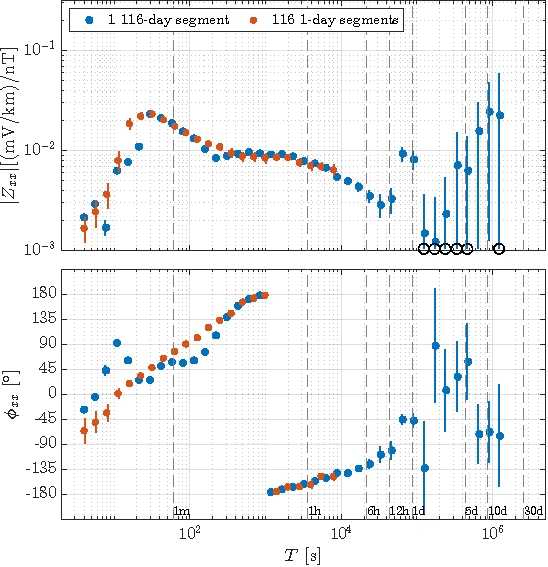
\includegraphics[width=0.48\textwidth]{figures/zplot-magnitude_phase-Middelpos-tf1-Z_xx.pdf}} 
  \subfigure(b){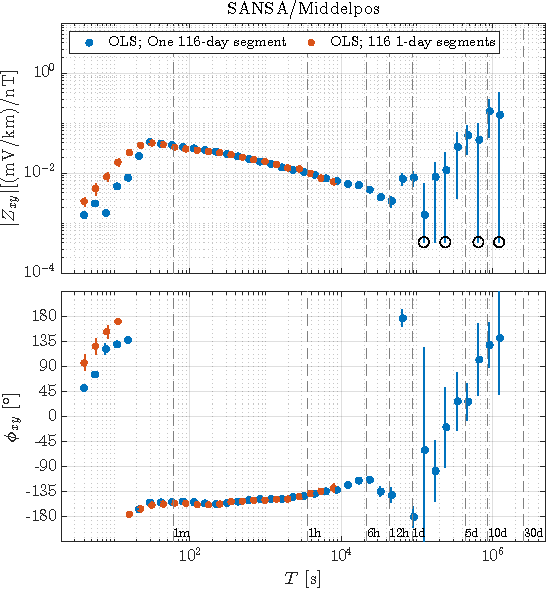
\includegraphics[width=0.48\textwidth]{figures/zplot-magnitude_phase-Middelpos-tf1-Z_xy.pdf}} 
  \subfigure(c){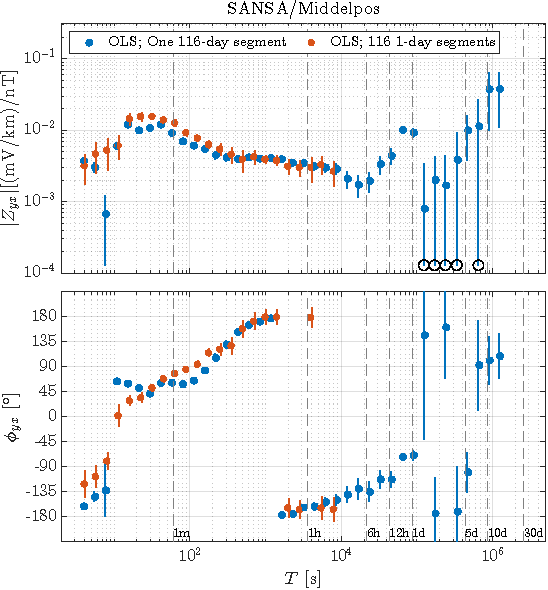
\includegraphics[width=0.48\textwidth]{figures/zplot-magnitude_phase-Middelpos-tf1-Z_yx.pdf}} 
  \subfigure(d){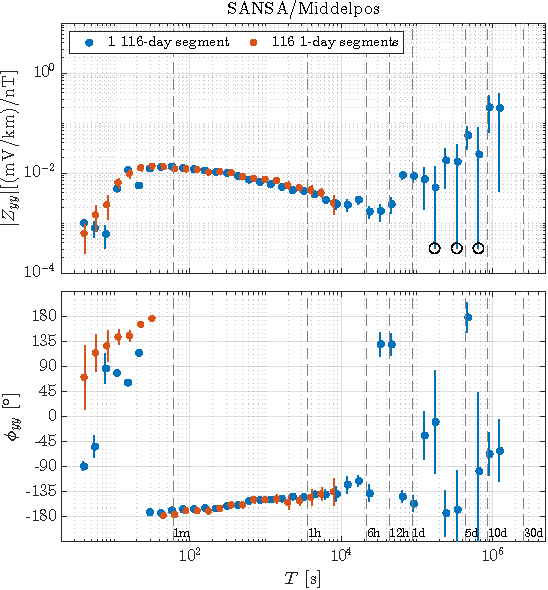
\includegraphics[width=0.48\textwidth]{figures/zplot-magnitude_phase-Middelpos-tf1-Z_yy.pdf}} 

  \caption{Magnitudes and phases for components of $\boldsymbol{\mathcal{Z}}$: (a) $Z_{xx}$ and $\phi_{xx}$; (b) $Z_{xy}$ and $\phi_{xy}$; (c) $Z_{yx}$ and $\phi_{yx}$; and (d) $Z_{yy}$ and $\phi_{yy}$. Open circles on the lower part of the impedance amplitude error bars indicate that this formula yielded a value below zero.}
    \label{fig:z}

  \subfigure(a){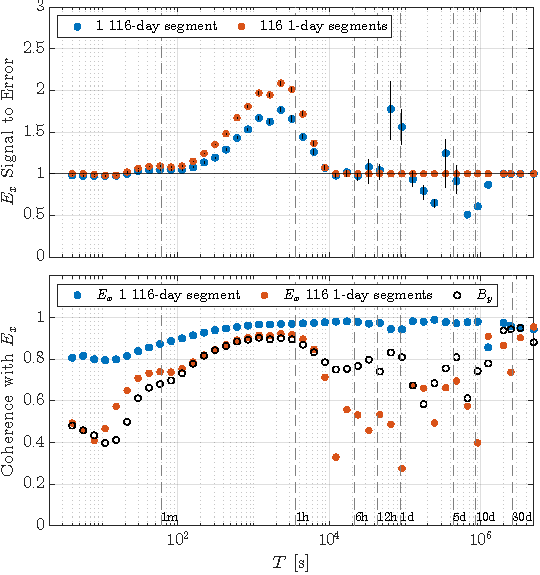
\includegraphics[width=0.48\textwidth]{figures/snplot-Middelpos-tf1-E_x.pdf}} 
  \subfigure(b){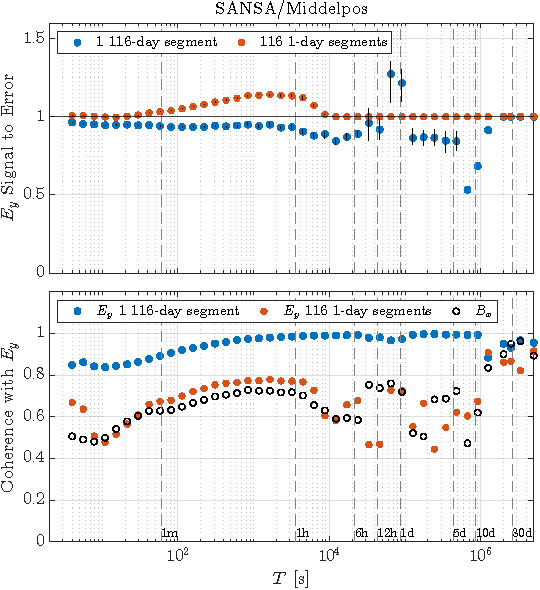
\includegraphics[width=0.48\textwidth]{figures/snplot-Middelpos-tf1-E_y.pdf}} 

  \caption{Model metrics for (a) $E_x$, corresponding to Figure~\ref{fig:z}(a)-(b) and (b) $E_y$, corresponding to Figure~\ref{fig:z}(b)-(c).}
  \label{fig:se}

\end{figure}

%\begin{figure}[h!] 
%\end{figure}

\clearpage

\section{Discussion}

\section{Appendix A}

\begin{figure}[h]
  \centering
  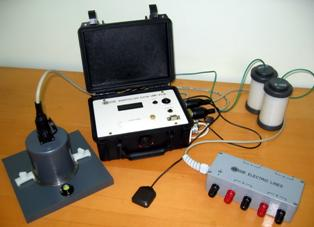
\includegraphics[width=0.5\textwidth]{figures/LEMI-417.jpg}
  \caption{LEMI-417 instrument (Manual: \url{https://www.ggki.hu/~novak/PRG/LEMI-417/LEMI-417UMrev7.pdf}; image from \url{https://www.isr.lviv.ua/lemi417.htm})}
  \label{fig:lemi}
\end{figure}

Figure~\ref{fig:lemi}: The Middelpos MT instrument. The LEMI-417 instrument and the 12V lead-acid batteries that power it are in a subterranean enclosure with concrete walls. The instrument is mounted on two 25-liter water bottles to reduce temperature variation. The solar panels are mounted on a steel frame over the enclosure. The side openings are covered with a canvas to prevent direct sunlight on the instrument. The small white dome above the solar panels is the GPS antenna.

\section{Appendix B}

\begin{table}
  \caption{Periods associated with evaluation frequency bands used for regression and smoothing spectra. \# is the evaluation frequency number, $N$ is the number of DFT points in the band, and $T_e\equiv 1/f_e$. The band range is from $T_l$ through $T_h$.}
  \centering
  \begin{tabular}{l l l l l}
    \hline \\
    \# & $N$ & $T_e$ [s] & $T_l$ [s] & $T_h$ [s] \\
    \hline \\
    1 & 2 & 43200 & 28800 & 86400 \\
    2 & 2 & 28800 & 21600 & 43200 \\
    3 & 3 & 21600 & 14400 & 43200 \\
    4 & 4 & 14400 & 9600 & 28800 \\
    5 & 5 & 10800 & 7200 & 21600 \\
    6 & 6 & 7854.5 & 5400 & 14400 \\
    7 & 8 & 5760 & 3927.3 & 10800 \\
    8 & 12 & 3927.3 & 2618.2 & 7854.5 \\
    9 & 16 & 2880 & 1920 & 5760 \\
    10 & 22 & 2009.3 & 1350 & 3927.3 \\
    11 & 31 & 1440 & 960 & 2880 \\
    12 & 43 & 1016.5 & 680.3 & 2009.3 \\
    13 & 61 & 720 & 480 & 1440 \\
    14 & 85 & 511.2 & 341.5 & 1016.5 \\
    15 & 120 & 361.5 & 241.3 & 720 \\
    16 & 170 & 255.6 & 170.4 & 511.2 \\
    17 & 240 & 180.8 & 120.5 & 361.5 \\
    18 & 338 & 128 & 85.4 & 255.6 \\
    19 & 478 & 90.5 & 60.3 & 180.8 \\
    20 & 676 & 64 & 42.7 & 128 \\
    21 & 956 & 45.2 & 30.2 & 90.5 \\
    22 & 1351 & 32 & 21.3 & 64 \\
    23 & 1910 & 22.6 & 15.1 & 45.2 \\
    24 & 2701 & 16 & 10.7 & 32 \\
    25 & 3819 & 11.3 & 7.5 & 22.6 \\
    26 & 5401 & 8 & 5.3 & 16 \\
    27 & 7638 & 5.7 & 3.8 & 11.3 \\
    28 & 10801 & 4 & 2.7 & 8 \\
    \hline \\
  \end{tabular}
  \label{evaluationperiods}
\end{table}

\clearpage

\bibliography{main.bib}

\end{document}
